\chapter{Contexte général du projet}
%\chapter{Présentation de l’entreprise}
Dans ce chapitre,nous présenterons le contexte général du projet qui sera décliné en deux parties : la premiére présentera la société d'accueil, et la seconde décrira le contexte,la  problématique,l'objectif attendu du projet ainsi que les fonctionnalités à mettre un place et la  planification de projet.                                                                                                                                                                                                                                                                                                                                                                                                                                                                                                                                                                                                                                                                                                                                                                                                                                                                                                          
\label{chap:introduction}
\section{Présentation de l'organisme d'accueil}
%\pagenumbering{arabic}
%\subsection{Introduction}
\begin{figure}[h]
	
\includegraphics[scale=0.14]{./Template LaTeX/Images/cado_logo.png}
	\centering
	\caption{CADOROM}
\end{figure}
CADORIM est une société de transfert d’argent mauritanienne basée à Nouakchott,
fondée fin 2018 par un entrepreneur mauritanien, titulaire d'un doctorat en
mathématiques,
CADORIM consiste a transférer de l’argent depuis n’importe quel pays dans le
monde vers ses proches en Mauritanie. Notre objectif et de fourni une plateforme
numérique permet à l’utilisateur de régler ses commandes en toute sécurité et
confidentialité assurée par le service de PayPal qui est mondialement connu pour sa
fiabilité et simplicité.t Pour effectuer un paiement il suffit d'une simple carte bancaire
ou un compte PayPal . et une éventuelle possibilité de virement bancaire.
CADORIM a été élu comme le champion de Banque Centrale de Mauritanie (BCM )
1ère édition 2019 Fintech Challenge,
Le siège social de CADORIM est situé à marche capital , Nouakchott, Mauritanie,
immatriculée au registre du commerce.
\subsection{Missions}
CADORIM offre une large palette de prestations organisées autour des activités suivantes :
\begin{enumerate}
	
	\item Maintenance et amélioration de leurs propres applications (CadoRim et MauriPay)
	\item Développement des applications 
	\item Des agences des reçoivent d'argent et de service client
	
\end{enumerate}
\subsection{Organigramme}
La structure organisationnelle de CADORIM comprend :
\begin{figure}[h]
	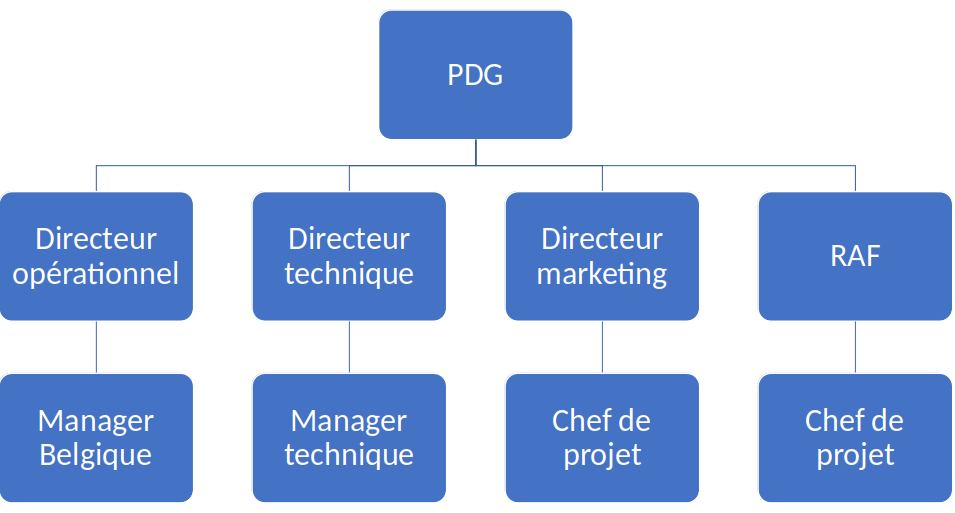
\includegraphics[scale=0.8,width=400px]{./Template LaTeX/Images/og.png}
	\centering
	\caption{Organigramme du CADORIM}
\end{figure}
\begin{enumerate}
	\item \textbf{PDG : }Le président directeur général qui coiffe toutes les unités de la société et qui définit la vision stratégique
	à adopter en vue de pleinement remplir leurs missions.
	\item \textbf{Directeur opérationnel :} Il joue un rôle d’intermédiaire et d’interface entre les différents services de CADORIM. Il assure un réel lien entre les équipes de Service et les clients.
	\item \textbf{Directeur technique :} Il joue le rôle de l'encadrant des équipes techniques (recruter, animer, motiver et faire adhérer) et suivre la veille technologique.
	\item \textbf{Directeur marketing :} Occupe un rôle stratégique et de management. Il s’occupe de la conception des produits, mais aussi de la présentation des offres qui ont pour but de satisfaire les consommateurs.
	\item \textbf{RAF :} Le responsable administratif, comptable et financier est l’un des hommes-clés .le RAF doit assurer la gestion financière, administrative et même comptable.
	
	
	\item \textbf{Manager :}Le rôle du manager  et des cadres (leadership) est d’assurer un lien cohérent entre les équipes.
	%\item \textbf{Manager Belgique :}
	%\item \textbf{Manager technique :}
	\item \textbf{Chef de projet :} Le chef de projet organise et conduit le projet. Il assume la responsabilité des différentes phases, depuis la traduction des besoins utilisateurs en spécifications fonctionnelles et techniques, jusqu'à la recette utilisateur, voire la mise en production.
\end{enumerate}
\begin{comment}
	content...

\subsection{Planification du projet}
J'effectuais le diagramme de Gantt, pour avoir une meilleure compréhension de la chronologie des étapes de mon projet.
\newline
\newline
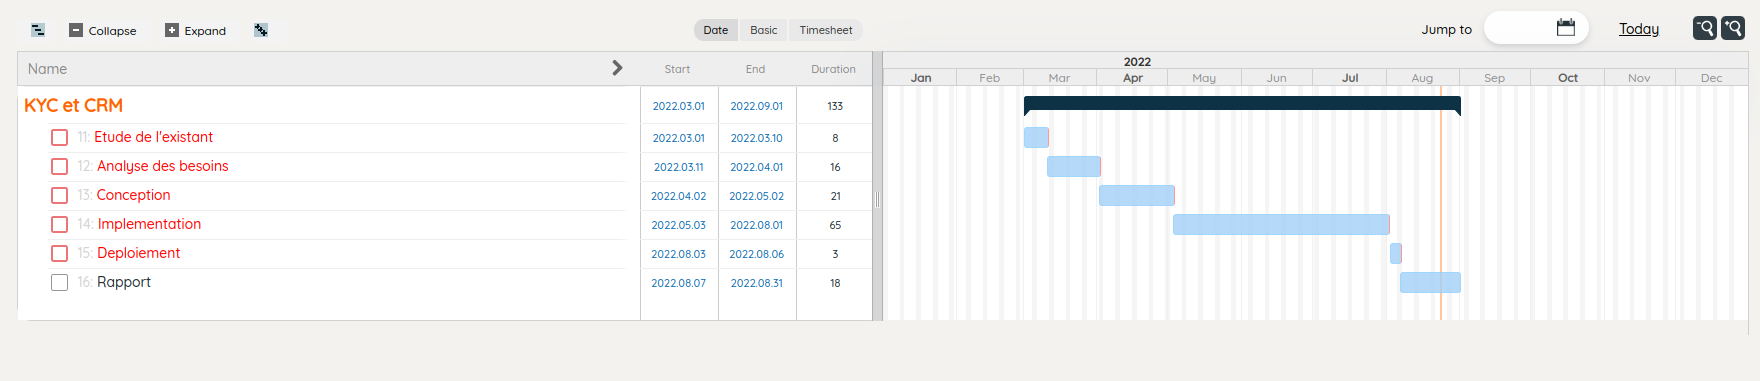
\includegraphics[width=500px,height=175px]{./Template LaTeX/Images/gantt.png}
\newline
Le projet est subdivisé en plusieurs phases.
\begin{enumerate}
\item Une phase comprenant l’étude de l’existant et analyse des besoins, en
intervenant les différents acteurs du projet.
\item Une phase de conception consistant à modéliser et formaliser les
données brutes du cahier de charge
\item Une phase d’implémentation consiste à traduire techniquement les
données provenant de la conception.
\item Déploiement : externalisation des ressources.
\end{enumerate}
\end{comment}

\section{Cadre général du projet}
%%%%%%%%%%%%%%%%%%%%%%%%%%%%%%%%%%%%% New add from Introduction %%%%%%%%%%%%%%%%%%%%%
\begin{comment}
	content...

Savoir qui est votre client et adopter des protocoles pour prévenir la criminalité financière sont des défis permanents pour les institutions financières. De manière significative, les institutions financières (y compris les banques, les coopératives de crédit et les sociétés financières du Fortune 50) doivent se conformer à un ensemble des réglementations de plus en plus complexes pour la vérification de l'identité des clients appelée KYC.

KYC, également connu sous le nom de "Know Your Customer" ou "Know Your Client", est un ensemble de procédures permettant de vérifier l'identité d'un client avant ou pendant les transactions avec les banques et autres institutions financières. Le respect des réglementations KYC peut aider à tenir à distance le blanchiment d'argent, le financement du terrorisme et d'autres stratagèmes de fraude courants. En vérifiant d'abord l'identité et les intentions d'un client au moment de l'ouverture du compte, puis en comprenant ses habitudes de transaction, les institutions financières sont en mesure d'identifier plus précisément les activités suspectes. 

Les institutions financières sont soumises à des normes de plus en plus strictes en matière de lois KYC. Ils doivent dépenser plus d'argent pour se conformer à KYC ou être passibles de lourdes amendes. Ces réglementations signifient que presque toutes les entreprises, plateformes ou organisations qui interagissent avec une institution financière pour ouvrir un compte ou effectuer des transactions devront se conformer à ces obligations.

La gestion de la relation client (CRM) est la combinaison de pratiques, de stratégies et de technologies que les entreprises utilisent pour gérer et analyser les interactions et les données client tout au long du cycle de vie du client. L'objectif est d'améliorer les relations de service client, de contribuer à la fidélisation de la clientèle et de stimuler la croissance des ventes. Les systèmes CRM compilent les données client à travers différents canaux, ou points de contact, entre le client et l'entreprise, qui peuvent inclure le site Web de l'entreprise, le téléphone, le chat en direct, le publipostage, les supports marketing et les réseaux sociaux. Les systèmes CRM peuvent également donner aux membres du personnel en contact avec les clients des informations détaillées sur les informations personnelles des clients, l'historique des achats, les préférences et les préoccupations d'achat.


\subsection{Motivations}    

KYC est un moyen de rendre la vérification de l'identité des clients plus précise et moins vulnérable à la fraude.

KYC doivent être effectuées lors de l'intégration d'un nouveau client, mais il est préférable de répéter ces vérifications de temps en temps, pour s'assurer que tout est comme il se doit. En surveillant les comptes clients de cette manière, les comportements suspects peuvent être signalés plus rapidement.

Un système CRM fournit des flux de travail automatisés qui permettent à votre équipe marketing de consacrer plus de temps à des tâches stratégiques, telles que la création de campagnes marketing qui résonnent, l'analyse des données de ces campagnes et le test de différentes approches basées sur ces analyses. Les agents du service client peuvent passer leur temps à travailler avec des clients qui ont des questions, des problèmes ou des besoins plus complexes. En bref, avec des processus de service client plus efficaces, les entreprises peuvent établir de meilleures relations avec leurs clients.
\end{comment}
\subsection{Problématique }	

\begin{comment}
	content...

En réalité, la réalisation d'une application,qui applique le principe de KYC et integre un  système CRM,
nécessite
de faire face à des problématiques diverses et complexes. Ainsi, la société a décidé de se contenter,
dans un premier temps, Mise en place d’un système d’extration des donnees à partir des images (carte d'identité ou passeport) et traitement des ces donnees.
Ce sujet soulève de nombreuses questions aux implications différentes. Comment peut extraire le texte apartir de l'image? Comment sera-t-il traité ? Comment peut-il être utilisé dans le principe KYC ? Comment pouvons-nous obtenir un système CRM intégré ?


Pour illustrer la couverture contre le risque de la fraude(de blanchiment, identité…),les sanctions(à cause du non respect de la réglementation),le risque juridique et fiscal.
Et puisque que les sociétés  réalisent facilement plus de ventes grâce à l’utilisation d’un system CRM(Gestion de la Relation Client).
\newline
Agissant avec lucidité et consciente des évolutions que connaît son domaine
\end{comment}
%Afin de lutter contre la fraude financière et de réaliser plus de ventes
Afin de résoudre le problème de fraude financière et réaliser plus des ventes, la société CADORIM a décidé de développer deux systèmes l'un pour lutte contre les fraudes financières, les usurpations d’identité, le blanchiment et il permet aussi de mieux connaître ses clients et d’en analyser les risques.
En plus il  est aussi bien sûr un gage de sécurité supplémentaire offerte aux clients contre toute usurpation d’identité ou détournement d’un compte CADORIM. ce system quand il est bien implémenté, permet non seulement de prévenir les fraudes mais il va également améliorer l’expérience client en  rendant la vérification des informations plus simple et fluide, ce system est connue sous le nom KYC.
Et l'autre collecte, enregistre et classifie les données liées aux clients d’une entreprise. Ses fonctionnalités permettent de gérer certains processus des fonctions ventes, clientèle et marketing.
CRM permettant à une entreprise d'obtenir :
\begin{itemize}[label=$\ast$]
\item Une base de données clients partagée.
\item Une plate-forme de travail pour les services commerciaux et marketing.
\item Une source d’indicateurs quantitatifs pour piloter la gestion de l’activité.
\end{itemize}

\subsection{Objectifs du projet}

\begin{comment}
La mise en place d'une application pour appliquer l'ide de KYC en basant sur les différent technologie disponible . En basan sur l'extraction du text apartir d'une imange OCR on peut extracter la code MRZ apartir d'une imange du piece d'idendite ou passport est passe le code a un algorithem qui permer de d'etecter les information personnel.
\newpage
\end{comment}
L’objectif principal du projet est de concevoir et développer une solution mobile dont le but est
de faciliter aux futurs utilisateurs la gestion de transfert d’argent. Le résultat de ce travail doit répondre aux objectifs fixés.
Notre objectif général se décompose en différents objectifs spécifiques à savoir :
\begin{itemize}[label=$\ast$]
	\item \textbf{Faciliter le parcours d'inscription :} Le client renseigne un certain nombre d’informations via un formulaire. Ensuite, le client scan un document d’identité, via la caméra de son smartphone . Les informations sont ensuite analysées automatiquement.
	
	\item \textbf{Faciliter  le transfert d’argent :} Avec son téléphone, l’utilisateur pourra
	envoyer l'argent à tout moment sans perdre du temps.
	
	
	\item \textbf{Réduire  les coûts de transfert :} Avec une telle solution, l’idée est de
	pouvoir envoyer de petites sommes d’argent donc il n’y aura pas lieu de payer des frais de transfert  exorbitants.
	
	
	\item \textbf{Participer à la diversification des services de transfert d’argent :}Vu le nombre de
	système de transfert d’argent déjà existant, l’idée n’est pas ici d’être leur concurrent
	mais plutôt un complément des services qui sont sur le marché pour une bonne
	satisfaction des clients.
	
	
	\item \textbf{Ajouter une fenêtre de discussion  :}Pour améliorer l'expérience client .

\end{itemize}
%\subsection{Fonctionnalités à mettre en place }
\subsection{Planification du projet}
\begin{center}
	
		\begin{table}[h]
			
		\hspace*{-2cm}
		%\vspace*{6cm}
		\begin{tabular}{|m{0.5cm}|m{6.5cm}|m{4cm}|m{3cm}|m{4cm}|}
			\hline
			\textbf{N°} &\textbf{Phase} & \textbf{Date début}&\textbf{Durée}& \textbf{Date de fin}
			\\
			\hline
			1
			&
			Découverte de produit et stratégie 
			&2022/03/01
			&8 jours
			&2022/03/10
			\\
			\hline
			2
			&
			Planification du processus de conception
			&2022/03/11
			&12 jours
			&2022/03/28
			\\
			\hline
			3
			&
			Idéation
			&2022/03/29
			&25 jours
			&2022/05/02
			\\
			\hline
			4
			&
			Conception et développement
			&2022/05/03
			&65 jour
			&2022/08/01
			\\
			\hline
			5
			&
			Test de l’application
			&2022/08/03
			&3 jour
			&2022/08/06
			\\
			\hline
			6
			&
			Activités pré-lancement
			&2022/08/08
			&4 jour
			&2022/08/12
			\\
			\hline
			7
			&	
			Rapport
			&2022/08/15
			&13 jour
			&2022/08/31
			\\
			\hline
		\end{tabular}
	
		%\vspace*{10cm}
		\centering \caption{Planification du projet}
		\label{fig4:classT}
	\end{table}

	
	
	
	
	
	
	
	
	
	
	
	
	%%%%%%%%%%%%%%%%%%%%%%%%%%%%%%%%
	\begin{comment}
	
	\begin{table}[h]
		%\hspace*{-2cm}
		%\vspace*{6cm}
		\begin{tabular}{|m{4.5cm}|m{4cm}|m{4cm}|m{4cm}|}
			\hline
			\textbf{Phase} & \textbf{Date début}&\textbf{Durée}& \textbf{Date de fin}
			\\
			\hline
			\textbf{Etude de l'existant:}  
					\begin{enumerate}
					\item[•]a
					\item[•]b
					\item[•]c
					\item[•]d
				\end{enumerate}
			&\hspace{0.97cm}2022/03/01
				\begin{enumerate}
				\item[]2022/03/01
				\item[]b
				\item[]c
				\item[]d
			\end{enumerate}	
			&\hspace{0.97cm}8 jour
				\begin{enumerate}
				\item[]8 jour
				\item[]b
				\item[]c
				\item[]d
			\end{enumerate}
			&\hspace{0.97cm}2022/03/10
				\begin{enumerate}
				\item[]2022/03/10
				\item[]b
				\item[]c
				\item[]d
			\end{enumerate}
			\\
			\hline
			\textbf{Analyse des besoins:}  
			\begin{enumerate}
				\item[•]a
				\item[•]b
				\item[•]c
				\item[•]d
			\end{enumerate}
			&\hspace{0.97cm}2022/03/11
			\begin{enumerate}
				\item[]2022/03/01
				\item[]b
				\item[]c
				\item[]d
			\end{enumerate}	
			&\hspace{0.97cm}16 jour
			\begin{enumerate}
				\item[]8 jour
				\item[]b
				\item[]c
				\item[]d
			\end{enumerate}
			&\hspace{0.97cm}2022/04/01
			\begin{enumerate}
				\item[]2022/03/10
				\item[]b
				\item[]c
				\item[]d
			\end{enumerate}
			\\
			\hline
			\textbf{Conception:}  
			\begin{enumerate}
				\item[•]a
				\item[•]b
				\item[•]c
				\item[•]d
			\end{enumerate}
			&\hspace{0.97cm}2022/03/01
			\begin{enumerate}
				\item[]2022/03/01
				\item[]b
				\item[]c
				\item[]d
			\end{enumerate}	
			&\hspace{0.97cm}8 jour
			\begin{enumerate}
				\item[]8 jour
				\item[]b
				\item[]c
				\item[]d
			\end{enumerate}
			&\hspace{0.97cm}2022/03/10
			\begin{enumerate}
				\item[]2022/03/10
				\item[]b
				\item[]c
				\item[]d
			\end{enumerate}
			\\
			\hline
			\textbf{Implementation:}  
			\begin{enumerate}
				\item[•]a
				\item[•]b
				\item[•]c
				\item[•]d
			\end{enumerate}
			&\hspace{0.97cm}2022/03/01
			\begin{enumerate}
				\item[]2022/03/01
				\item[]b
				\item[]c
				\item[]d
			\end{enumerate}	
			&\hspace{0.97cm}8 jour
			\begin{enumerate}
				\item[]8 jour
				\item[]b
				\item[]c
				\item[]d
			\end{enumerate}
			&\hspace{0.97cm}2022/03/10
			\begin{enumerate}
				\item[]2022/03/10
				\item[]b
				\item[]c
				\item[]d
			\end{enumerate}
			\\
			\hline
			\textbf{Deploiement:}  
			\begin{enumerate}
				\item[•]a
				\item[•]b
				\item[•]c
				\item[•]d
			\end{enumerate}
			&\hspace{0.97cm}2022/03/01
			\begin{enumerate}
				\item[]2022/03/01
				\item[]b
				\item[]c
				\item[]d
			\end{enumerate}	
			&\hspace{0.97cm}8 jour
			\begin{enumerate}
				\item[]8 jour
				\item[]b
				\item[]c
				\item[]d
			\end{enumerate}
			&\hspace{0.97cm}2022/03/10
			\begin{enumerate}
				\item[]2022/03/10
				\item[]b
				\item[]c
				\item[]d
			\end{enumerate}
			\\
			\hline
			 & & &
				\end{tabular}
		%\vspace*{10cm}
	\centering \caption{Planification du projet}
\label{fig4:classT}
\end{table}
	\begin{table}[h]
	%\hspace*{-2cm}
	\vspace*{-6.6cm}
	\begin{tabular}{|m{4.5cm}|m{4cm}|m{4cm}|m{4cm}|}

			
			\textbf{Rapport:}  
			\begin{enumerate}
				\item[•]a
				\item[•]b
				\item[•]c
				\item[•]d
			\end{enumerate}
			&\hspace{0.97cm}2022/03/01
			\begin{enumerate}
				\item[]2022/03/01
				\item[]b
				\item[]c
				\item[]d
			\end{enumerate}	
			&\hspace{0.97cm}8 jour
			\begin{enumerate}
				\item[]8 jour
				\item[]b
				\item[]c
				\item[]d
			\end{enumerate}
			&\hspace{0.97cm}2022/03/10
			\begin{enumerate}
				\item[]2022/03/10
				\item[]b
				\item[]c
				\item[]d
			\end{enumerate}
			\\
			\hline
		\end{tabular}
		%\vspace*{10cm}
		\centering \caption{Planification du projet}
		\label{fig4:classT}
	\end{table}
	content...
\end{comment}
%%%%%%%%%%%%%%%%%%%%%%%%%%%%%%%%%%
\end{center}
Dans le cadre de la conduite du projet, la réalisation d'un planning à suivre tout au long du stage de fin d'études est indispensable. Ainsi, le stage a débuté le mardi 1 mars 2022. En conséquence, une réunion s'est tenue afin de définir le calendrier du projet.
\begin{center}
%	\hspace*{-2.5cm}
		\begin{ganttchart}[
		hgrid,
		vgrid={*{6}{draw=none}, dotted},
		x unit=0.092cm,
		time slot format=isodate,
		time slot unit=day,
		calendar week text = {\currentweek{}},
		bar height = 1, %necessary to make it fit the height
		bar top shift = -0.01, %to move it inside the grid space ;)
		]{2022-03-01}{2022-08-31}
		\gantttitlecalendar{year, month=name, week} \\
		\ganttbar[bar/.append style={fill=cyan}]{ 1}{2022-03-01}{2022-03-10}\\
		\ganttbar[bar/.append style={fill=cyan}]{ 2}{2022-03-11}{2022-03-28}\\
		\ganttbar[bar/.append style={fill=cyan}]{3}{2022-03-29}{2022-05-02}\\
		\ganttbar[bar/.append style={fill=cyan}]{ 4}{2022-05-03}{2022-08-01}\\
		\ganttbar[bar/.append style={fill=cyan}]{5}{2022-08-03}{2022-08-06}\\
		\ganttbar[bar/.append style={fill=cyan}]{ 6}{2022-08-08}{2022-08-12}\\
		\ganttbar[bar/.append style={fill=cyan}]{7}{2022-08-15}{2022-08-31}
	\end{ganttchart}
		
	%\hspace*{-2.5cm}
		\begin{comment}
		content...
	\begin{ganttchart}[y unit title=0.4cm,
	y unit chart=0.5cm,
	vgrid,hgrid,
	title height=1,
	bar/.style={draw,fill=cyan},
	bar incomplete/.append style={fill=yellow!50},
	bar height=0.7]{1}{27}
	\gantttitle{Mars}{5}
	\gantttitle{Avril}{3}
	\gantttitle{Mai}{5}
	\gantttitle{Juin}{5}
	\gantttitle{Juillet}{4}
	\gantttitle{Aout}{5}
	 \\
	\gantttitlelist{1,...,27}{1}\\
	%\gantttitlelist{5,...,6}{1} \\
	\ganttbar{Etude de l'existant}{1}{2/5} \\
	\ganttbar{Analyse des besoins}{5/2}{9/2} \\
	\ganttbar{Conception}{9/2}{10} \\
	\ganttbar{Implementation}{10}{23} \\
	\ganttbar{Deploiement}{23}{24} \\
	\ganttbar{Rapport}{24}{27} \\
%	\ganttbar[progress=70]{Fase 3}{13}{18} \\
%	\ganttbar[progress=40]{Conclus\~ao}{20}{24} \\
	% rela\c c\~oes
%	\ganttlink{elem0}{elem1}
%	\ganttlink{elem1}{elem2}
%	\ganttlink{elem2}{elem3}
\end{ganttchart}
\end{comment}
\end{center}

\begin{comment}

\begin{figure}[h]
	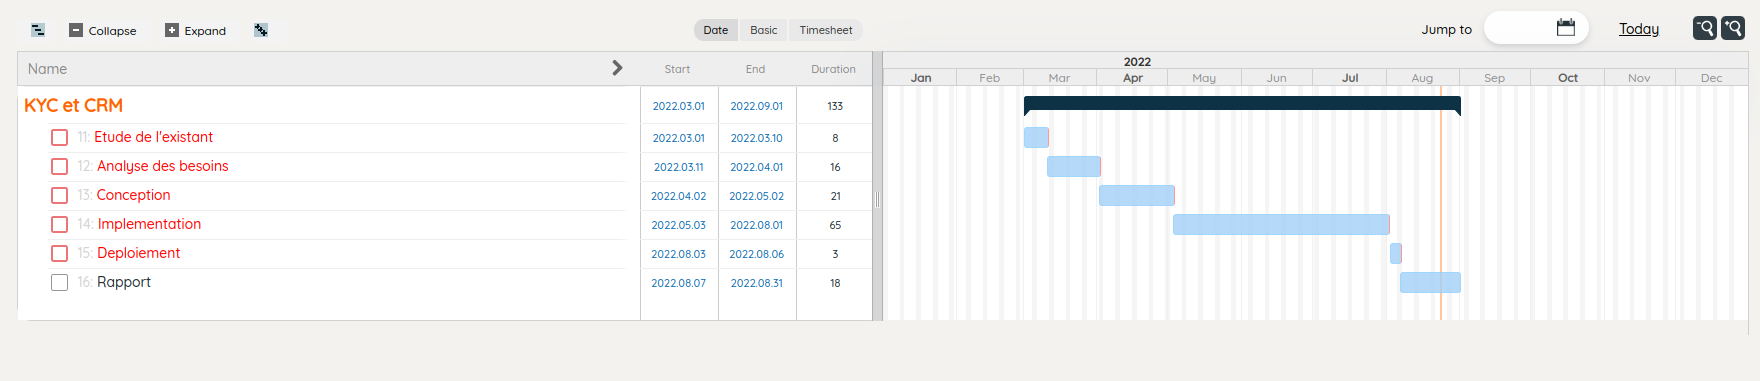
\includegraphics[scale=0.8,width=500px,height=175px]{./Template LaTeX/Images/gantt.png}
	\centering
	\caption{Diagramme de Gantt du projet}
\end{figure}
	content...
	\newpage


Le projet est subdivisé en plusieurs phases.
\begin{enumerate}
	\item Une phase comprenant l’étude de l’existant et analyse des besoins, en
	intervenant les différents acteurs du projet.
	\item Une phase de conception consistant à modéliser et formaliser les
	données brutes du cahier de charge
	\item Une phase d’implémentation consiste à traduire techniquement les
	données provenant de la conception.
	\item Déploiement : externalisation des ressources.
\end{enumerate}
\end{comment}
\begin{enumerate}
	\item L'objectif de la phase de découverte du produit est de connaître nos utilisateurs finaux afin de comprendre leurs besoins et être en mesure de leur proposer la solution adaptée, en priorisant les fonctionnalités essentielles. La définition d'une stratégie de produit est une partie essentielle du processus, car elle nous aidera à garder nos objectifs commerciaux à l'esprit à chaque étape du développement de notre produit final.
	
	
	\item La deuxième phase consiste à rédiger une feuille de route produit qui nous aidera à définir les éléments essentiels de la conception de la note produit et à les regrouper en différentes étapes de livraison. de cette manière, nous obtiendrons un plan précis des différents composants de notre produit et des délais dans lesquels chacun doit être complété. 
	
	
	
	
	
	\item La phase d'idéation consiste à explorer différentes idées créatives pour atteindre les objectifs du projet. C'est là qu'une ligne directrice doit être établie, qui sera suivie à toutes les étapes du processus de développement.
	
	
	
	\item Le succès d'une application dépend de la réaction du public ciblé . Le design est une étape clé dans le processus de développement d'une application, car il définit non seulement le design de votre application, mais aussi et surtout son fonctionnement pour les utilisateurs finaux. Une application qui offre une excellente expérience utilisateur a de meilleures chances de succès.
	
	
	\item La phase de test permet de s'assurer que notre produit fonctionne correctement et qu'il est fiable, utilisable et agréable. Les tests peuvent être divisés en deux groupes principaux : les tests fonctionnels et non fonctionnels.\newline
	\textbf{-Tests fonctionnels : }Pour optimiser les tests fonctionnels, il convient de mettre en place un processus d'intégration continue. L'intégration continue automatise les tests à chaque fois que le code source change.\newline
	\textbf{-Tests non fonctionnels : }Les tests non fonctionnels vérifient les performances ou l'utilisabilité d'un produit. L'idée de base est de vérifier si le produit offre un design d'interaction efficace pour ses utilisateurs. Les tests d'utilisabilité peuvent être effectués de manière formelle, avec un chercheur créant une série de tâches, recrutant des participants, menant des sessions de tests et les enregistrant, etc., ou de manière plus informelle sous la forme de tests de guérilla. .
	
	
	\item Le développement d'une application est un processus itératif, qui ne s'arrête pas une fois l'application lancée. Après le développement, nous devons obtenir les commentaires de l'équipe technique et consacrer du temps et des ressources à l'amélioration de l'expérience utilisateur (UX). Cela vous aidera également à évaluer le succès à long terme de notre application.
	
	\item Préparation d'un rapport pour la documentation de travail.
\end{enumerate}

